\section{Evaluation}
\label{sec:evaluation}
We answer the research questions stated in Section~\ref{sec:intro}. \Den{As RQs agora estão em lista na introdução. Continua a sugestão de reorganização: RQ1 = rótulos (prevalência, taxa de falha, sensibilidade à rodada), que sustenta todo o resto; RQ2 = predição (CV + LOPO + baselines, incluindo o baseline só com o nome do repositório); RQ3 = vocabulário + comparação com outras linguagens; RQ4 = erros.}

\myparagraph{Rationale} RQ1.1 establishes whether the lexical trace of flakiness is strong enough, in C\#, for standard classifiers to separate flaky from stable tests using only static features, since the method has never been evaluated for a language with this concurrency model. RQ1.2 tests the labeling strategy: the conclusions of RQ1.1 hold only if the labels, which come from reruns and therefore from a nondeterministic process, are reasonably stable. RQ2 puts the results in context against trivial and structural baselines, to ensure that performance reflects genuine discriminative power rather than an artifact of the evaluation. RQ3 addresses interpretability: which lexical units drive the prediction, so they can be related to known root causes. RQ4 examines representative errors, to understand the limits of lexical prediction and when a static detector should or should not be trusted.

\subsection{Experimental setup}
\label{sec:setup}
Because the dataset is highly imbalanced (0.24\% flaky), a model that answered ``stable'' for everything would be right more than 99\% of the time without learning anything. We therefore evaluate in two stages. In the first, we train on a random undersample of the stable tests, so that each draw has as many stable tests as flaky ones (1:1 ratio), and apply stratified 5-fold cross-validation. We repeat the process with 10 different draws, yielding 50 estimates per model, and report the mean with a 95\% interval, which reflects variation across draws and folds but not uncertainty about other projects. Since the evaluation folds are also balanced, precision and F1 are inflated (a predictor that always answers ``flaky'' already obtains an F1 of 0.67). We therefore compare models by the Matthews correlation coefficient (MCC), which ranges from $-1$ to 1 with 0 at chance, and by the area under the ROC curve (AUC), the probability that a randomly drawn flaky test receives a higher score than a randomly drawn stable one. AUC does not depend on a decision threshold, which suits the use we propose, ranking tests to decide which to rerun first. \Den{O IC de 95\% sobre 50 estimativas correlacionadas (os mesmos 30 positivos em todas) é otimista. Usar o teste t corrigido de Nadeau e Bengio para CV repetida e comparar modelos com Wilcoxon pareado + $\delta$ de Cliff, ou Scott-Knott ESD (requer execução). Hoje nenhuma afirmação ``A é melhor que B'' tem teste de significância, e os revisores vão pedir.}

In the second stage, we evaluate what happens when facing a new project, since cross-validation mixes tests from all repositories and may reward the model merely for recognizing conventions of a project it has already seen. We use the leave-one-repository-out (LOPO) scheme: we train on all repositories but one and test on all tests of the held-out repository. We score the nine repositories that have flaky tests, which hold 7,758 labeled methods, so the natural proportion of flaky tests is 0.39\%. \Den{Na prática não se sabe de antemão quais repositórios têm flaky, então os demais (cerca de 4.900 testes) deveriam entrar nas métricas pooled (taxa 0.24\%), com os falsos alarmes neles reportados (requer execução). O AUC por repositório só é definido com positivos, mas AP e precisão pooled não precisam disso.} In this scenario, the closest to real use, we report average precision (AP) in addition to AUC. AP averages, over the flaky tests, the precision of the ranking at the position where each one is found, so it is high when flaky tests are concentrated at the top of the list. Unlike AUC, AP is sensitive to the rarity of positives: a model with no ranking power obtains an AP equal to the proportion of flaky tests, about 0.004. The difference between the results of the two stages indicates how much of the performance comes from general flakiness patterns and how much comes from each project's particular vocabulary.

As for implementation, Random Forest and Extra Trees use 200 trees; the SVM uses a linear kernel; KNN uses $k = 5$ with cosine distance; the remaining classifiers use scikit-learn's default values. In LOPO, training uses the same 1:1 undersampling of the other repositories (10 draws), the scores are the mean over the 10 draws, and the held-out repository is evaluated in full, at its natural class distribution. We report five complementary metrics in cross-validation (precision, recall, F1, MCC, and AUC) and four in LOPO (AUC, AP, recall, and precision). \Den{Precisão e recall no LOPO usam qual limiar? O padrão 0.5 de um modelo treinado com 1:1 é arbitrário na taxa natural. Para o uso proposto (ranking), reportar precision@$k$/recall@$k$ (top 10\%, top 25\%) ou uma métrica effort-aware (ex.: $P_{opt}$, recall@20\% do esforço, como em predição de defeitos), sempre também para os baselines.}

\subsection{RQ1.1 and RQ2: predictive effectiveness and baselines}
\label{sec:rq1}
In cross-validation, the ensemble models performed best: Extra Trees, Random Forest, and Gradient Boosting reach an MCC of 0.51--0.53 and an AUC of 0.83--0.87 (Table~\ref{tab:cv100}). The other classifiers range from 0.38 to 0.44 MCC, and the random and majority baselines stay at chance level. Two non-trivial baselines, however, are strong: the rule that uses only the ten most informative tokens reaches an MCC of 0.40, and the Random Forest that uses only the test's structure (without vocabulary) reaches 0.36. Relative to the structure-only model, vocabulary adds about 0.15--0.17 MCC for the best models, and less for the others (from 0.02 to 0.08); relative to the threshold rule, the gain of the ensembles is smaller (0.11--0.13). Since the structure-only model already counts \texttt{await} expressions, part of the lexical signal is present in both. \Den{Falta um teste estatístico pareado para estes ganhos (requer execução).} Part of the threshold rule's strength comes from project-specific tokens (Section~\ref{sec:rq3}); even so, the rule remains competitive across repositories (Table~\ref{tab:lopo}).

\begin{table}[!h]
\caption{Cross-validation with 100-run labels (mean $\pm$ 95\% CI; balanced test folds with about 6 flaky tests each). Best classifier per column in bold.}
\label{tab:cv100}
\centering
\scriptsize
\setlength{\tabcolsep}{2pt}
\begin{tabular}{@{}p{50pt}ccccc@{}}
\toprule
\textbf{Model} & \textbf{Prec.} & \textbf{Rec.} & \textbf{F1} & \textbf{MCC} & \textbf{AUC} \tabularnewline
\midrule
\raggedright Extra Trees            & \textbf{0.87}${\pm}$0.04 & 0.63${\pm}$0.06 & 0.69${\pm}$0.04 & \textbf{0.53}${\pm}$0.05 & 0.86${\pm}$0.03 \tabularnewline
\raggedright Random Forest          & 0.83${\pm}$0.04 & 0.64${\pm}$0.05 & 0.70${\pm}$0.04 & 0.51${\pm}$0.06 & \textbf{0.87}${\pm}$0.03 \tabularnewline
\raggedright Grad.\ Boosting        & 0.80${\pm}$0.04 & \textbf{0.70}${\pm}$0.05 & \textbf{0.72}${\pm}$0.04 & 0.51${\pm}$0.06 & 0.83${\pm}$0.03 \tabularnewline
\raggedright Logistic reg.          & 0.74${\pm}$0.04 & 0.69${\pm}$0.06 & 0.70${\pm}$0.04 & 0.44${\pm}$0.08 & 0.82${\pm}$0.03 \tabularnewline
\raggedright SVM                    & 0.73${\pm}$0.05 & \textbf{0.70}${\pm}$0.05 & 0.70${\pm}$0.04 & 0.43${\pm}$0.08 & 0.81${\pm}$0.03 \tabularnewline
\raggedright Naive Bayes            & 0.74${\pm}$0.04 & 0.69${\pm}$0.05 & 0.69${\pm}$0.04 & 0.43${\pm}$0.07 & 0.79${\pm}$0.04 \tabularnewline
\raggedright KNN                    & 0.71${\pm}$0.05 & 0.67${\pm}$0.06 & 0.67${\pm}$0.04 & 0.38${\pm}$0.07 & 0.74${\pm}$0.04 \tabularnewline
\raggedright Decision Tree          & 0.76${\pm}$0.05 & 0.66${\pm}$0.06 & 0.68${\pm}$0.05 & 0.44${\pm}$0.09 & 0.71${\pm}$0.04 \tabularnewline
\midrule
\multicolumn{6}{@{}l}{\emph{Baselines}} \tabularnewline
\raggedright Vocab.\ threshold      & 0.66${\pm}$0.04 & 0.87${\pm}$0.03 & 0.74${\pm}$0.02 & 0.40${\pm}$0.07 & 0.77${\pm}$0.03 \tabularnewline
\raggedright Structure only         & 0.68${\pm}$0.04 & 0.67${\pm}$0.06 & 0.66${\pm}$0.04 & 0.36${\pm}$0.07 & 0.73${\pm}$0.04 \tabularnewline
\raggedright Random                 & 0.52${\pm}$0.05 & 0.51${\pm}$0.05 & 0.50${\pm}$0.04 & 0.02${\pm}$0.08 & 0.53${\pm}$0.05 \tabularnewline
\raggedright Majority               & 0.50${\pm}$0.00 & 1.00${\pm}$0.00 & 0.67${\pm}$0.00 & 0.00${\pm}$0.00 & 0.50${\pm}$0.00 \tabularnewline
\bottomrule
\end{tabular}
\end{table}

Error profiles differ across models. The tree ensembles are the most precise (Extra Trees: precision 0.87 and recall 0.63), that is, when they flag a test as flaky they are usually right, but they miss some of them. The vocabulary threshold rule does the opposite: it has the highest recall (0.87) but a precision of only 0.66, lower than that of every trained classifier, because it flags as flaky any test containing the most informative tokens. The linear models, Naive Bayes, and KNN improve little or not at all over the structure-only model. Since the folds are balanced, these precisions do not transfer to real use, which the cross-repository validation quantifies.

In cross-repository validation (Table~\ref{tab:lopo}), which uses the natural flaky rate (0.39\%), AUC drops to 0.75--0.78 (macro and pooled) and precision is only 2--3\% for the two best models: for every flaky test found, there are dozens of false alarms. The pooled average precision (AP) of the two best models is four to six times the natural rate, which serves as the chance reference. This shows that the ranking is informative, but that automatic gating would be unusable. On pooled AP, however, the vocabulary rule is the strongest of all (0.025, against 0.023 for Random Forest and 0.015 for Extra Trees), although the tree ensembles lead on AUC. Macro AP is fragile with so few positives per repository: the macro AP of Random Forest (0.089) is driven by Testcontainers, whose single flaky test is ranked near the top (AP 0.507, Table~\ref{tab:lopo-repo}), and without it falls to about 0.036; logistic regression also has a higher macro AP than Extra Trees (0.065 vs.\ 0.055). \Den{Para comparar com a regra sem o Testcontainers, é preciso o AP da regra por repositório (incluir na Tab.~\ref{tab:lopo-repo}). Sugiro também reportar a mediana por repositório.}

\begin{table}[!h]
\caption{Cross-repository validation (LOPO) at the natural rate (0.39\%). Macro: mean over the nine repositories with flaky tests; pooled: all held-out tests together.}
\label{tab:lopo}
\centering
\scriptsize
\setlength{\tabcolsep}{3.5pt}
\begin{tabular}{@{}lrrrrrr@{}}
\toprule
 & \multicolumn{4}{c}{\textbf{Macro}} & \multicolumn{2}{c}{\textbf{Pooled}} \\
\cmidrule(lr){2-5}\cmidrule(lr){6-7}
\textbf{Model} & \textbf{AUC} & \textbf{AP} & \textbf{Rec.} & \textbf{Prec.} & \textbf{AUC} & \textbf{AP} \\
\midrule
Extra Trees          & 0.757 & 0.055 & 0.376 & 0.028 & 0.775 & 0.015 \\
Random Forest        & 0.754 & 0.089 & 0.376 & 0.021 & 0.753 & 0.023 \\
Gradient Boosting    & 0.709 & 0.048 & 0.509 & 0.012 & 0.734 & 0.021 \\
Logistic regression  & 0.679 & 0.065 & 0.574 & 0.009 & 0.741 & 0.017 \\
SVM                  & 0.660 & 0.048 & 0.556 & 0.010 & 0.730 & 0.015 \\
Naive Bayes          & 0.644 & 0.053 & 0.567 & 0.009 & 0.718 & 0.018 \\
KNN                  & 0.597 & 0.020 & 0.529 & 0.008 & 0.711 & 0.011 \\
Decision Tree        & 0.597 & 0.011 & 0.476 & 0.012 & 0.740 & 0.010 \\
\midrule
\multicolumn{7}{@{}l}{\emph{Baselines}} \\
Vocabulary threshold  & 0.682 & 0.040 & 0.732 & 0.008 & 0.721 & 0.025 \\
Structure only        & 0.674 & 0.020 & 0.559 & 0.009 & 0.654 & 0.006 \\
Random                & 0.516 & 0.013 & 0.507 & 0.005 & 0.554 & 0.006 \\
Majority              & 0.500 & 0.005 & 1.000 & 0.005 & 0.500 & 0.004 \\
\bottomrule
\end{tabular}
\end{table}

Table~\ref{tab:lopo-repo} shows the variation across repositories for the two best models. AUC ranges from 0.53 (NetMQ, with 2 flaky tests) to 0.97 (Testcontainers, with 1); repositories with a single flaky test (Akka.NET, Quartz.NET, and Testcontainers) are only illustrative. Among those with several flaky tests, Nerdbank.Streams is the most favorable (AUC of 0.74 to 0.80 and AP of 0.15 to 0.18), while MassTransit and StreamJsonRpc, which together hold 14 of the 30 flaky tests, have AUCs of 0.67 to 0.70. Figure~\ref{fig:auc} summarizes the main effect: for every model, AUC drops when the test's repository is not part of training; the drop is smaller for the tree ensembles (about 0.10 to 0.12) than for logistic regression, SVM, Naive Bayes, and KNN (0.14 to 0.15).

\Den{Tab.~\ref{tab:lopo-repo}: MassTransit aparece com 1.548 testes, mas a Tab.~\ref{tab:projetos} soma 1.209 casos (76 + 1.133), e o número de métodos declarantes não pode ser maior que o de casos. Conferir esta coluna (ver também Nerdbank e StreamJsonRpc no comentário da Tab.~\ref{tab:armadilhas}). Incluir as linhas da regra e do baseline estrutural para a comparação por repositório.}
\begin{table}[!h]
\caption{Per-repository LOPO for the two best models (RF: Random Forest; ET: Extra Trees). Repositories with a single flaky test are only illustrative.}
\label{tab:lopo-repo}
\centering
\scriptsize
\setlength{\tabcolsep}{4pt}
\begin{tabular}{@{}lrrrrrr@{}}
\toprule
 & & & \multicolumn{2}{c}{\textbf{RF}} & \multicolumn{2}{c}{\textbf{ET}} \\
\cmidrule(lr){4-5}\cmidrule(lr){6-7}
\textbf{Repository} & \textbf{Flaky} & \textbf{Tests} & \textbf{AUC} & \textbf{AP} & \textbf{AUC} & \textbf{AP} \\
\midrule
Akka.NET         & 1 & 1,134 & 0.782 & 0.006 & 0.862 & 0.008 \\
MassTransit      & 6 & 1,548 & 0.672 & 0.023 & 0.704 & 0.019 \\
Nerdbank.Streams & 6 &   595 & 0.795 & 0.179 & 0.741 & 0.154 \\
NetMQ            & 2 &   259 & 0.530 & 0.015 & 0.549 & 0.017 \\
NLog             & 2 & 1,692 & 0.844 & 0.009 & 0.834 & 0.009 \\
Polly            & 3 &   559 & 0.775 & 0.033 & 0.846 & 0.041 \\
Quartz.NET       & 1 & 1,016 & 0.737 & 0.004 & 0.646 & 0.003 \\
StreamJsonRpc    & 8 &   763 & 0.681 & 0.020 & 0.696 & 0.022 \\
Testcontainers   & 1 &   192 & 0.969 & 0.507 & 0.933 & 0.223 \\
\bottomrule
\end{tabular}
\end{table}

\begin{figure}[!h]
\centering
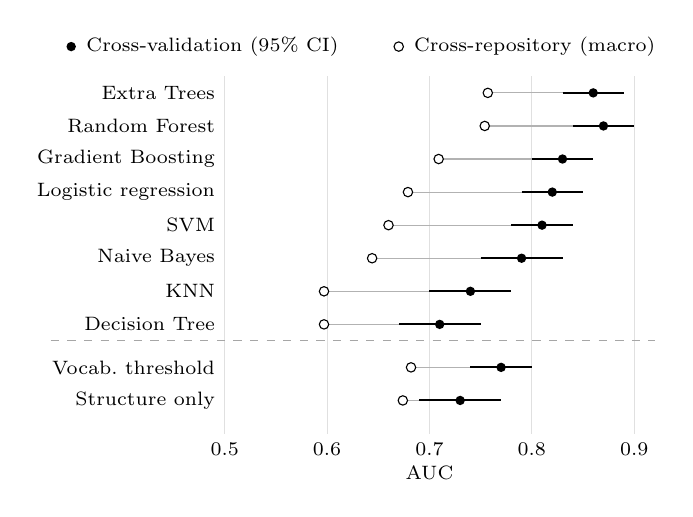
\begin{tikzpicture}[x=13cm, y=0.42cm, font=\scriptsize]
  % x coordinate = AUC - 0.5
  \foreach \t in {0.5,0.6,0.7,0.8,0.9} {
    \draw[black!12] ({\t-0.5},0.5) -- ({\t-0.5},-10.3);
    \node[below] at ({\t-0.5},-10.3) {\t};
  }
  \node at (0.2,-11.5) {AUC};
  \draw[dashed, black!35] (-0.17,-7.5) -- (0.42,-7.5);
  \foreach \y/\name/\cv/\ci/\lo in {
      0/Extra Trees/0.86/0.03/0.757,
      1/Random Forest/0.87/0.03/0.754,
      2/Gradient Boosting/0.83/0.03/0.709,
      3/Logistic regression/0.82/0.03/0.679,
      4/SVM/0.81/0.03/0.660,
      5/Naive Bayes/0.79/0.04/0.644,
      6/KNN/0.74/0.04/0.597,
      7/Decision Tree/0.71/0.04/0.597,
      8.3/Vocab.\ threshold/0.77/0.03/0.682,
      9.3/Structure only/0.73/0.04/0.674} {
    \node[left] at (0,-\y) {\name};
    \draw[black!30] ({\lo-0.5},-\y) -- ({\cv-0.5},-\y);
    \draw[line width=0.7pt] ({\cv-\ci-0.5},-\y) -- ({\cv+\ci-0.5},-\y);
    \fill ({\cv-0.5},-\y) circle (1.7pt);
    \draw[fill=white] ({\lo-0.5},-\y) circle (1.7pt);
  }
  \fill (-0.15,1.4) circle (1.7pt) node[right=2pt] {Cross-validation (95\% CI)};
  \draw[fill=white] (0.17,1.4) circle (1.7pt) node[right=2pt] {Cross-repository (macro)};
\end{tikzpicture}
\caption{AUC under cross-validation (filled, with 95\% CI; balanced folds) and macro AUC across repositories (hollow), by model and baseline. The axis starts at 0.5, the chance level.}
\label{fig:auc}
\end{figure}

\noindent\fbox{\parbox{\dimexpr\columnwidth-2\fboxsep-2\fboxrule\relax}{\textbf{RQ1.1 and RQ2:} vocabulary predicts flakiness in C\# well above chance (MCC 0.51--0.53, AUC 0.86--0.87 under cross-validation; AUC 0.75--0.78 across repositories), but its advantage is moderate: about $+$0.15 MCC over a structure-only model that already counts \texttt{await} expressions, only for the tree ensembles, and a ten-token rule matches the models on pooled AP across repositories. The practical value lies in ranking.}}

\subsection{RQ1.2: label robustness}
\label{sec:rq12}
The two rerun rounds diverge (Table~\ref{tab:sobreposicao}): of the 36 flaky units found by either of them, only 13 are flaky in both (Jaccard 0.36); 17 are flaky only in the 100-run round and 6 only in the 20-run round. The 20-run round finds 43\% of what the 100-run round finds, and the 100-run round finds 68\% of what the 20-run round finds. Part of this divergence is expected from the number of runs alone: a test that fails once in 100 runs has only about an 18\% chance of failing at least once in 20. Since a single flip on the same version shows that a test is flaky, all 36 units are flaky, and the divergence measures how many flaky tests each round misses rather than how many it gets wrong. \Den{Com a taxa de falha $p$ de cada teste na rodada de 100, somar $1-(1-p)^{20}$ para os 30 testes dá a sobreposição esperada, que pode ser comparada com os 13 observados (requer os dados de k/100). Treinar com o rótulo união (36) como análise adicional também requer execução.} Most tests exclusive to the 100-run round fail rarely (for example, Nerdbank.Streams 6$\to$0, NetMQ 2$\to$0), and of the six exclusive to the 20-run round, four are in NLog and three of them failed together in a single run, so they represent a single event. One of the tests exclusive to the 100-run round failed in all 20 controlled runs, which suggests an environmental difference between the rounds. \Den{Esse teste é \emph{broken} na rodada de 20, o que reforça que as rodadas diferem também no ambiente (SDK?), e não só no número de execuções. Investigar a causa (versão do SDK? dependência de data?) e reportar.} In LOPO with the 20-run labels, only five repositories have flaky tests, and the best macro AUC is 0.72. \Den{Este número não aparece em nenhuma tabela; incluir na Tab.~\ref{tab:cv100x20} ou no artefato.} With the 20-run labels (Table~\ref{tab:cv100x20}), the tree ensembles lose 0.07 to 0.14 MCC and 0.04 to 0.12 AUC, and the structure-only model (MCC 0.47) catches up with them within the confidence interval; the advantage of vocabulary holds only with the richer labels. \Den{A Tab.~\ref{tab:cv100x20} não mostra os ICs mencionados (``within the confidence interval''); incluí-los.}

\begin{table}[!h]
\caption{Overlap between the flaky units of the two rounds.}
\label{tab:sobreposicao}
\centering
\footnotesize
\begin{tabular}{@{}lcp{0.50\columnwidth}@{}}
\toprule
\textbf{Category} & \textbf{Units} & \textbf{Where} \tabularnewline
\midrule
Flaky in both & 13 & \raggedright StreamJsonRpc 5, MassTransit.Tests 3, Polly 2, Akka.NET 1, MassTransit.Abstractions 1, NLog 1 \tabularnewline[2pt]
Only in 100 runs & 17 & \raggedright Nerdbank.Streams 6, StreamJsonRpc 3, NetMQ 2, MassTransit.Tests 2, Testcontainers 1, Quartz 1, NLog 1, Polly 1 \tabularnewline[2pt]
Only in 20 runs & 6 & \raggedright NLog 4, MassTransit.Tests 1, Polly 1 \tabularnewline
\bottomrule
\end{tabular}
\end{table}

\begin{table}[!h]
\caption{Cross-validation with 100-run vs.\ 20-run labels (19 flaky units in the latter).}
\label{tab:cv100x20}
\centering
\footnotesize
\setlength{\tabcolsep}{5pt}
\begin{tabular}{@{}lcccc@{}}
\toprule
 & \multicolumn{2}{c}{\textbf{MCC}} & \multicolumn{2}{c}{\textbf{AUC}} \\
\cmidrule(lr){2-3}\cmidrule(lr){4-5}
\textbf{Model} & \textbf{100$\times$} & \textbf{20$\times$} & \textbf{100$\times$} & \textbf{20$\times$} \\
\midrule
Extra Trees       & 0.53 & 0.43 & 0.86 & 0.82 \\
Random Forest     & 0.51 & 0.44 & 0.87 & 0.80 \\
Gradient Boosting & 0.51 & 0.37 & 0.83 & 0.71 \\
\midrule
\multicolumn{5}{@{}l}{\emph{Baselines}} \\
Vocab.\ threshold & 0.40 & 0.23 & 0.77 & 0.66 \\
Structure only    & 0.36 & 0.47 & 0.73 & 0.77 \\
Random            & 0.02 & 0.04 & 0.53 & 0.54 \\
\bottomrule
\end{tabular}
\end{table}

As an independent check, the six tests flaky only in the 20-run round are labeled stable under the 100-run labels and receive a score when their own repository is held out, so the model has never seen them as positives. Three of them rank in the top 15\% of their repository (percentiles 0.96, 0.95, and 0.85), and the three NLog tests that failed together fall at percentiles 0.30--0.42. Counting the trio as a single event, three of four independent events are ranked high. With only four events, this check is anecdotal, but it points in the same direction as the cross-repository results.

\medskip
\noindent\fbox{\parbox{\dimexpr\columnwidth-2\fboxsep-2\fboxrule\relax}{\textbf{RQ1.2:} the lexical signal persists across rounds, but whether it beats structure depends on the round that produced the labels. The round changes which tests are flaky (Jaccard 0.36), largely because 20 runs miss rarely failing tests, and with the 20-run labels the structure-only model matches the ensembles.}}
\medskip

\subsection{RQ3: the vocabulary of flaky tests in C\#}
\label{sec:rq3}
Table~\ref{tab:tokens} shows the tokens with the highest information gain that occur in flaky tests from at least three repositories. The most informative markers are Task-based concurrency, that is, operations run in the background and awaited with \texttt{async}/\texttt{await} (\texttt{task} in 80\% of flaky tests vs.\ 31\% of stable ones; \texttt{async}/\texttt{await} in 67\% vs.\ 30\%), time handling (\texttt{TimeSpan}, \texttt{CancellationToken}, \texttt{Sleep}, \texttt{Delay}), and resource lifecycles (\texttt{Dispose}, \texttt{StopAsync}), along with rare, specific markers such as \texttt{GC} and \texttt{WeakReference} (Table~\ref{tab:marcadores}). This is consistent with the asynchronous-wait and concurrency causes reported for other languages \cite{luo2014empirical, barbosa2023test} and with the sleep/timeout pattern described for .NET \cite{leesatapornwongsa2022flakerepro}. The frequent markers are general: \texttt{task}, \texttt{async}, and \texttt{await} occur in six repositories. However, a third of stable tests in C\# also contain \texttt{async}/\texttt{await}, which explains why presence rules are weak. \Den{(i) Uma comparação sistemática com os vocabulários de Java, JS e Swift (ver o comentário da introdução sobre uma RQ cross-language) sustentaria a frase sobre consistência com outras linguagens, que suavizei. (ii) Os números ``80\% vs.\ 31\%'' e ``67\% vs.\ 30\%'' não estão na Tab.~\ref{tab:tokens}, que não tem a coluna \%S.}

\Den{Tab.~\ref{tab:tokens}: adicionar \%S, o número de repositórios e o lift (requer os dados; tirei o \%S da legenda porque a coluna não existe). Explicar tokens pouco intuitivos como \texttt{length}, \texttt{enumerable} e \texttt{writeline} (este pode refletir saída de log/diagnóstico, não uma causa). O filtro ``$\geq$3 repositórios'', aplicado depois de ver o ranking bruto, pode parecer \emph{cherry-picking}: mostrar o ranking bruto (no artefato ou numa coluna) e justificar o critério \emph{a priori}.}
\begin{table}[!h]
\caption{Top tokens by information gain (IG, in nats) present in flaky tests from at least three repositories. \%F: proportion of the 30 flaky units containing the token.}
\label{tab:tokens}
\centering
\footnotesize
\setlength{\tabcolsep}{12pt}
\begin{tabular}{@{}lrr@{}}
\toprule
\textbf{Token} & \textbf{IG} & \textbf{\%F} \\
\midrule
\texttt{task}              & 0.145 & 80 \\
\texttt{async task}        & 0.084 & 67 \\
\texttt{await}             & 0.084 & 67 \\
\texttt{async}             & 0.082 & 67 \\
\texttt{length}            & 0.065 & 27 \\
\texttt{await task}        & 0.061 & 23 \\
\texttt{server}            & 0.056 & 23 \\
\texttt{enumerable}        & 0.044 & 13 \\
\texttt{logger}            & 0.044 & 20 \\
\texttt{fromseconds}       & 0.043 & 20 \\
\texttt{writeline}         & 0.038 & 17 \\
\texttt{timespan}          & 0.034 & 23 \\
\texttt{dispose}           & 0.034 & 13 \\
\texttt{cancellationtoken} & 0.025 & 13 \\
\bottomrule
\end{tabular}
\end{table}

The raw information-gain ranking is dominated by project conventions: \texttt{trait}, \texttt{fact trait}, and \texttt{checkgcpressureasync} come only from StreamJsonRpc, and \texttt{trait} originates from an attribute, not from the test body. This dominance is itself evidence that part of what the models learn is the identity of the project (Section~\ref{sec:discussion}). Information gain favors frequent tokens; we therefore also report rare but specific markers by lift (Table~\ref{tab:marcadores}). They fall into memory and garbage collection (\texttt{gc}, \texttt{weakreference}), asynchronous composition (\texttt{whenall}), cancellation (\texttt{cancellationtokensource}), lifecycles (\texttt{stopasync}, \texttt{disposed}), and fixed waits (\texttt{sleep}, \texttt{task delay}). Each occurs in only two to four flaky tests, so they are exploratory. \Den{O IG leave-one-project-out (comentário no Step~6) quantificaria a dominância de StreamJsonRpc (requer execução).}

\Den{Tab.~\ref{tab:marcadores}: explicar os ``---'' (por que só alguns tokens foram testados?). O lift com 2 ocorrências é instável; considerar um IC ou suavização (lift com pseudo-contagem). Conferi que o menor $p$ (\texttt{gc}, $\approx 10^{-5}$) não sobrevive a Bonferroni ($\approx 10^{-6}$), e isso agora está na legenda.}
\begin{table}[!h]
\caption{Rare, specific markers (at least two flaky tests in at least two repositories, except \texttt{weakreference}). $p$-values: one-sided Fisher's exact tests; none survives a Bonferroni correction for the roughly 48,000 candidate tokens, so the table is exploratory.}
\label{tab:marcadores}
\centering
\scriptsize
\setlength{\tabcolsep}{5pt}
\begin{tabular}{@{}lrrrrr@{}}
\toprule
\textbf{Token} & \textbf{Flaky} & \textbf{\%F} & \textbf{\%S} & \textbf{\emph{Lift}} & \textbf{\emph{p}} \\
\midrule
\texttt{gc}                      & 3 & 10.0 & 0.12 & 84$\times$ & $<$0.001 \\
\texttt{weakreference}           & 2 &  6.7 & 0.18 & 37$\times$ & 0.002 \\
\texttt{stopasync}               & 2 &  6.7 & 0.12 & 56$\times$ & --- \\
\texttt{disposed}                & 2 &  6.7 & 0.13 & 50$\times$ & --- \\
\texttt{whenall}                 & 4 & 13.3 & 0.62 & 22$\times$ & --- \\
\texttt{cancellationtokensource} & 4 & 13.3 & 1.56 &  9$\times$ & --- \\
\texttt{sleep}                   & 2 &  6.7 & 0.82 &  8$\times$ & 0.03 \\
\texttt{task delay}              & 2 &  6.7 & 0.97 &  7$\times$ & 0.04 \\
\bottomrule
\end{tabular}
\end{table}

\myparagraph{Relation to root causes} The markers connect to the causes of flakiness described in the Introduction. \texttt{task}, \texttt{async}, and \texttt{await} indicate background operations whose completion the test must await, the territory of race conditions. \texttt{TimeSpan}, \texttt{FromSeconds}, \texttt{CancellationToken}, \texttt{Sleep}, and \texttt{Delay} indicate dependence on time and timeouts. \texttt{Dispose}, \texttt{StopAsync}, \texttt{server}, \texttt{logger}, and \texttt{WriteLine} indicate external resources that must be created and released, such as servers and output streams. \texttt{GC} and \texttt{WeakReference} indicate dependence on the garbage collector, whose timing is nondeterministic. This reading is an interpretation of the tokens, not a confirmed classification of each test's cause. \Den{Sugestão de alto impacto e baixo custo: com apenas 36 flaky, dá para rotular manualmente a causa raiz de cada um (taxonomia de Luo et al., dois avaliadores, kappa de Cohen) e cruzar categorias com tokens. Isso transforma a interpretação em evidência, responde à pergunta ``o vocabulário captura a causa?'' e é uma contribuição empírica nova para C\#.}

\myparagraph{Stability markers} Unlike Swift, where \texttt{xctassertequal} marks clearly synchronous tests, we found no robust stability marker: among the tokens present in flaky tests from at least three repositories, the only one more frequent in stable tests is \texttt{assert} (67\% vs.\ 69\%), which does not discriminate. The token \texttt{areequal} (0\% vs.\ 20\%) is an NUnit assertion style used by repositories without flaky tests, so it reflects the choice of framework, not stability. \Den{Conferir: a Seção~\ref{sec:subjects} diz que MassTransit e Quartz.NET usam NUnit e ambos têm flaky, então ``NUnit assertion style used by repositories without flaky tests'' não é exato (talvez eles usem \texttt{Assert.That}). De todo modo, o exemplo mostra que o modelo pode aprender framework/repositório, o que reforça a necessidade do baseline de repositório e da amostragem pareada.}

\medskip
\noindent\fbox{\parbox{\dimexpr\columnwidth-2\fboxsep-2\fboxrule\relax}{\textbf{RQ3:} flakiness in C\# is signaled by \texttt{Task}-based concurrency, time handling, and resource lifecycles, complemented by rare markers such as \texttt{GC} and \texttt{WeakReference}. The frequent markers are general across repositories, the rare ones are specific but backed by few tests, the raw ranking is dominated by the conventions of a single project, and no robust stability marker emerged.}}
\medskip

\subsection{RQ4: error analysis}
\label{sec:rq4}
To analyze errors, we use the LOPO scores, in which each test is scored by models trained without its repository. The score is the mean of Random Forest and Extra Trees over the 10 undersampling draws. In each of the nine repositories that have flaky tests, we rank all labeled tests (flaky and stable) by score, breaking ties by average rank, and compute each test's percentile within its repository, so that 1.0 corresponds to the highest-scoring test. The 30 flaky tests have a median percentile of 0.80; 9 have a percentile of at least 0.90, that is, they are in the top 10\% of their repository, 23 have a percentile of at least 0.75, in the top 25\%, and 6 fall below the median. This means that, if each repository were ranked by the model and the top quartile were selected for rerunning (about a quarter of the tests), that quartile would contain 77\% of the flaky tests, against about 25\% expected by chance, with a 95\% Clopper--Pearson confidence interval of 58\% to 90\%. \Den{\textbf{Falta o mais importante: comparar com os baselines na mesma métrica} (requer execução). Pela Seção~\ref{sec:rq3}, o token \texttt{task} sozinho está em 80\% dos flaky e em 31\% dos estáveis: rerodar só os testes com \texttt{task} cobre $\approx$80\% dos flaky com $\approx$31\% do esforço, quase o mesmo custo-benefício do modelo (77\% com 25\%). É preciso mostrar a curva recall vs.\ fração rerodada para o modelo, a regra, o estrutural, \texttt{task}/\texttt{async} e o aleatório. Se o modelo não ganhar com clareza da regra de um token, a recomendação de usar o ranking para priorizar reruns fica frágil.} The result also does not depend on the repositories that concentrate the positives: in the three largest (20 of the 30 flaky tests), 14 are in the top quartile (70\%), and in the other six repositories, 9 of 10 (90\%), although these have only one or two each.

This estimate should be read with caution. The two models that make up the score were chosen for their performance on the same data, and the confidence interval treats tests as independent, even though they come from a convenience sample and some are correlated (three NLog tests failed together), so the real uncertainty is probably larger. We also assume the same execution cost per test, which probably underestimates the real cost, since asynchronous tests and tests with fixed waits tend to be slower. Moreover, the result measures how concentrated flaky tests are at the top of the ranking, not the chance that rerunning reveals the flakiness, which depends on how often each test fails.

We also examined, in the test source code, the errors for the tests the model did not place in the top quartile (seven of the 30) and for the highest-scoring stable tests. \Den{Descrever o protocolo: quantos estáveis de maior score foram examinados (top-10 por repositório?), quem analisou (um ou dois autores?) e como as divergências foram resolvidas. Dos 7 falsos negativos, só 5 são discutidos.} This is a qualitative analysis of a few examples, not a count of causes. The false negatives are flaky tests whose cause lies beyond the reach of vocabulary. Three patterns recur. (i) The test merely delegates to a helper method: \texttt{JsonRpcPerf\_Pipe} and \texttt{JsonRpcPerf\_Channel} (Nerdbank.Streams) are one-line calls to a shared helper, with no assertions, so the cause lies outside the test body; \texttt{InvokeWithProgressParameter\_\allowbreak NoMemoryLeakConfirm} (StreamJsonRpc) awaits a helper, forces \texttt{GC.Collect()}, and checks a \texttt{WeakReference}, and its nondeterminism comes from garbage collection. (ii) Fixed waits without asynchronous constructs: \texttt{ReconnectOnRouterBug} (Section~\ref{sec:motivation}) synchronizes only through \texttt{Thread.Sleep}, a token present in only two flaky tests and weakly learned. (iii) Time and global state: MassTransit's \texttt{Should\_be\_using\_the\_\allowbreak correct\_algorithm\_\allowbreak for\_sequential\_guids} installs a tick provider and compares parts of consecutively generated identifiers, which depends on the clock and, apparently, on shared static state.

The false positives are stable tests that use concurrency and time deterministically. Polly's \texttt{Execute\_CallerCancellation\_\allowbreak EnsureExceptionCarriesCallerToken} uses an injected time provider and a cancellation token, being asynchronous and time-related, yet deterministic by construction; Quartz's \texttt{Trigger\_Fires\_After\_Clock\_\allowbreak Jumps\_Backward\_And\_Returns} controls time through a custom provider and awaits a \texttt{TaskCompletionSource} instead of sleeping. The model detects the constructs but does not judge whether they are used well. Akka.NET's \texttt{A\_CircuitBreaker\_stress\_test} uses a fixed \texttt{await Task.Delay(3000)} with a wide margin and may be latently flaky beyond our 120 runs, so some false positives may be label noise. \Den{Experimento barato e convincente: rerodar os $\sim$20 falsos positivos de maior score de 500 a 1.000 vezes e/ou sob stress de CPU. Se alguns falharem, há evidência de que o modelo encontra flaky latentes (e de que os rótulos por rerun subestimam a flakiness), o que vira um resultado positivo forte.}

\medskip
\noindent\fbox{\parbox{\dimexpr\columnwidth-2\fboxsep-2\fboxrule\relax}{\textbf{RQ4:} the model fails when the cause is hidden in helper methods, in GC behavior, or in shared state (false negatives), and when asynchronous or time constructs are used with controlled time or event-based synchronization (false positives). Judging whether usage is correct requires semantic, not lexical, analysis.}}
\medskip

\subsection{Sensitivity analyses}
\label{sec:sensitivity}
We tested two threats to the vocabulary signal, keeping the labels, undersampling seeds, and folds fixed so that the comparison is paired. \Den{Se a comparação é pareada, aplicar um teste pareado (Wilcoxon sobre as 50 estimativas) e reportar $p$ e tamanho de efeito.} Without attributes: we removed all tokens inside attribute lists (\texttt{[Fact]}, \texttt{[Trait(...)]}, \texttt{[InlineData(...)]}), so that project conventions do not drive the prediction. With helpers: we added to each test the tokens of the helper methods it calls, resolved by name (at most five helpers per test, one level only); the expansion resolved at least one helper in 67\% of the methods, and, since resolution is by name, without type information, some helpers may merely share a name with the one actually called. \Den{O artigo já usa Roslyn: com o \texttt{SemanticModel}, resolver as chamadas com informação de tipo é direto e elimina a ambiguidade por nome. Como os helpers são o principal padrão de falso negativo (RQ4), essa melhoria tem ótimo custo-benefício e pode virar uma contribuição técnica.}

\begin{table}[!h]
\caption{Sensitivity of cross-validation MCC and LOPO macro AUC (original features, without attributes, with one-level helpers).}
\label{tab:sensibilidade}
\centering
\scriptsize
\setlength{\tabcolsep}{3.5pt}
\begin{tabular}{@{}lcccccc@{}}
\toprule
 & \multicolumn{3}{c}{\textbf{MCC (CV)}} & \multicolumn{3}{c}{\textbf{Macro AUC (LOPO)}} \\
\cmidrule(lr){2-4}\cmidrule(lr){5-7}
\textbf{Model} & \textbf{orig.} & \textbf{no attr.} & \textbf{+help.} & \textbf{orig.} & \textbf{no attr.} & \textbf{+help.} \\
\midrule
Extra Trees         & 0.53 & 0.46 & 0.56 & 0.757 & 0.737 & 0.764 \\
Random Forest       & 0.51 & 0.46 & 0.53 & 0.754 & 0.721 & 0.773 \\
Gradient Boosting   & 0.51 & 0.49 & 0.43 & 0.709 & 0.683 & 0.643 \\
Logistic regression & 0.44 & 0.43 & 0.49 & 0.679 & 0.673 & 0.714 \\
\midrule
\multicolumn{7}{@{}l}{\emph{Baseline}} \\
Structure only      & 0.36 & 0.36 & 0.36 & 0.674 & 0.674 & 0.674 \\
\bottomrule
\end{tabular}
\end{table}

Removing attributes reduces the MCC of the two best ensembles from 0.53 to 0.46 (Extra Trees) and from 0.51 to 0.46 (Random Forest), but keeps AUC at 0.84--0.85: \Den{Esses valores de AUC não estão na Tab.~\ref{tab:sensibilidade} (que mostra MCC da CV e AUC do LOPO). Incluir a coluna ou remover.} attributes carry part of the signal, plausibly project conventions, but most of it lies in the test body, and the ensembles remain well above the structure-only baseline. Adding helpers slightly improves the ensembles (MCC 0.56 and 0.53) and improves the linear and probabilistic models more, but hurts Gradient Boosting (from 0.51 to 0.43) and the Decision Tree (from 0.44 to 0.39). \Den{O Decision Tree não está na Tab.~\ref{tab:sensibilidade}. Incluir ou remover.} The ensembles' gains are within the confidence intervals. The naive one-level expansion therefore does not eliminate the helper blind spot: it adds tokens to two thirds of the tests, flaky or stable alike.
